\documentclass[10pt,a4paper,onecolumn]{article}
% \usepackage[utf8]{inputenc}
\usepackage{marginnote}
\usepackage{graphicx}
\usepackage{xcolor}
\usepackage{authblk,etoolbox}
\usepackage{titlesec}
\usepackage{calc}
\usepackage{hyperref}
\usepackage{amssymb,amsmath,array,amsthm}
\hypersetup{breaklinks=true,
            bookmarks=true,
            pdfauthor=
{
      Georgios Detorakis,
  },
            pdftitle=
{
[Re] A Generalized Linear Integrate-and-Fire Neural Model Produces Diverse
Spiking Behaviors
},
            colorlinks=true,
            citecolor=blue,
            urlcolor=blue,
            linkcolor=blue,
            pdfborder={0 0 0}}
\urlstyle{same}
\usepackage{tcolorbox}
\usepackage{ragged2e}
\usepackage{fontspec}
\usepackage{fontawesome}
\usepackage[singlelinecheck=off]{caption}
\usepackage{listings}
\lstnewenvironment{code}{\lstset{language=Haskell,basicstyle=\small\ttfamily}}{}



%\usepackage{fancyvrb}
%\VerbatimFootnotes
%\usepackage{graphicx}
%\usepackage{mdframed}
%\newmdenv[backgroundcolor=lightgray]{Shaded}


\usepackage{longtable,booktabs}

\usepackage[
  backend=biber,
%  style=alphabetic,
%  citestyle=numeric
]{biblatex}
\bibliography{bibliography.bib}



% --- Macros ------------------------------------------------------------------
\renewcommand*{\bibfont}{\small \sffamily}

\definecolor{red}{HTML}{CF232B}
\newcommand{\ReScience}{Re{\bfseries \textcolor{red}{Science}}}

\newtcolorbox{rebox}
   {colback=blue!5!white, colframe=blue!40!white,
     boxrule=0.5pt, arc=2pt, fonttitle=\sffamily\scshape\bfseries,
     left=6pt, right=20pt, top=6pt, bottom=6pt}

\newtcolorbox{repobox}
   {colback=red, colframe=red!75!black,
     boxrule=0.5pt, arc=2pt, left=6pt, right=6pt, top=3pt, bottom=3pt}

% fix for pandoc 1.14     
\newcommand{\tightlist}{%
  \setlength{\itemsep}{1pt}\setlength{\parskip}{0pt}\setlength{\parsep}{0pt}}

% --- Style -------------------------------------------------------------------
\renewcommand*{\bibfont}{\small \sffamily}
\renewcommand{\captionfont}{\small\sffamily}
\renewcommand{\captionlabelfont}{\bfseries}

\makeatletter
\renewcommand\@biblabel[1]{{\bf #1.}}
\makeatother

% --- Page layout -------------------------------------------------------------
\usepackage[top=3.5cm, bottom=3cm, right=1.5cm, left=1.5cm,
            headheight=2.2cm, reversemp, includemp, marginparwidth=4.5cm]{geometry}

% --- Section/SubSection/SubSubSection ----------------------------------------
\titleformat{\section}
  {\normalfont\sffamily\Large\bfseries}
  {}{0pt}{}
\titleformat{\subsection}
  {\normalfont\sffamily\large\bfseries}
  {}{0pt}{}
\titleformat{\subsubsection}
  {\normalfont\sffamily\bfseries}
  {}{0pt}{}
\titleformat*{\paragraph}
  {\sffamily\normalsize}


% --- Header / Footer ---------------------------------------------------------
\usepackage{fancyhdr}
\pagestyle{fancy}
%\renewcommand{\headrulewidth}{0.50pt}
\renewcommand{\headrulewidth}{0pt}
\fancyhead[L]{\hspace{-1cm}
\includegraphics[width=4.0cm]{rescience-logo.pdf}}
\fancyhead[C]{}
\fancyhead[R]{} 
\renewcommand{\footrulewidth}{0.25pt}

\fancyfoot[L]{\hypersetup{urlcolor=red}
              \sffamily \ReScience~$\vert$
              \href{http://rescience.github.io}{rescience.github.io}
              \hypersetup{urlcolor=blue}}
\fancyfoot[C]{\sffamily 7 - \thepage}
\fancyfoot[R]{\sffamily Oct 2017 $\vert$
                        Volume \textbf{3} $\vert$
                        Issue \textbf{1}}
\pagestyle{fancy}
\makeatletter
\let\ps@plain\ps@fancy
\fancyheadoffset[L]{4.5cm}
\fancyfootoffset[L]{4.5cm}

% --- Title / Authors ---------------------------------------------------------
% patch \maketitle so that it doesn't center
\patchcmd{\@maketitle}{center}{flushleft}{}{}
\patchcmd{\@maketitle}{center}{flushleft}{}{}
% patch \maketitle so that the font size for the title is normal
\patchcmd{\@maketitle}{\LARGE}{\LARGE\sffamily}{}{}
% patch the patch by authblk so that the author block is flush left
\def\maketitle{{%
  \renewenvironment{tabular}[2][]
    {\begin{flushleft}}
    {\end{flushleft}}
  \AB@maketitle}}
\makeatletter
\renewcommand\AB@affilsepx{ \protect\Affilfont}
%\renewcommand\AB@affilnote[1]{{\bfseries #1}\hspace{2pt}}
\renewcommand\AB@affilnote[1]{{\bfseries #1}\hspace{3pt}}
\makeatother
\renewcommand\Authfont{\sffamily\bfseries}
\renewcommand\Affilfont{\sffamily\small\mdseries}
\setlength{\affilsep}{1em}

\LetLtxMacro{\OldIncludegraphics}{\includegraphics}
\renewcommand{\includegraphics}[2][]{\OldIncludegraphics[width=12cm, #1]{#2}}


% --- Document ----------------------------------------------------------------
\title{[Re] A Generalized Linear Integrate-and-Fire Neural Model Produces Diverse
Spiking Behaviors}

    \usepackage{authblk}
                        \author[1]{Georgios Detorakis}
                            \affil[1]{Department of Cognitive Sciences, UC Irvine, Irvine CA, USA}
            
\date{\vspace{-5mm}
      \sffamily \small \href{mailto:gdetorak@uci.edu (gdetor@protonmail.com)}{gdetorak@uci.edu (gdetor@protonmail.com)}}


\setlength\LTleft{0pt}
\setlength\LTright{0pt}


\begin{document}
\maketitle

\marginpar{
  %\hrule
  \sffamily\small
  %\vspace{2mm}
  {\bfseries Editor}\\
  Tiziano Zito\\

  {\bfseries Reviewers}\\
        Hans Ekkehard Plesser\\
        Pierre de Buyl\\
  
  {\bfseries Received}  Aug, 3, 2017\\
  {\bfseries Accepted}  Aug, 18, 2017\\
  {\bfseries Published} Oct, 6, 2017\\

  {\bfseries Licence}   \href{http://creativecommons.org/licenses/by/4.0/}{CC-BY}

  \begin{flushleft}
  {\bfseries Competing Interests:}\\
  The authors have declared that no competing interests exist.
  \end{flushleft}

  \hrule
  \vspace{3mm}

  \hypersetup{urlcolor=white}
  
    \vspace{-1mm}
  \begin{repobox}
    \bfseries\normalsize
      \href{https://github.com/ReScience-Archives/Detorakis-2017}{\faGithubAlt~Article repository}
  \end{repobox}
      \vspace{-1mm}
  \begin{repobox}
    \bfseries\normalsize
      \href{https://github.com/ReScience-Archives/Detorakis-2017}{\faGithubAlt~Code repository}
  \end{repobox}
        \hypersetup{urlcolor=blue}
}

\begin{rebox}
\sffamily {\bfseries A reference implementation of}
\small
\begin{flushleft}
\begin{itemize}
    \item[→] A Generalized Linear Integrate-and-Fire Neural Model Produces Diverse
Spiking Behaviors, Stefan Mihalas and Ernst Niebur, Neural Computation
21, 704--718, 2009.
  \end{itemize}\par
\end{flushleft}
\end{rebox}


\section{Introduction}\label{introduction}

Integrate-and-fire neurons are being used extensively in the field of
neuroscience for modeling spiking behaviors~\autocite{dayan:2001}. In
this work we provide a reference implementation
of~\autocite{mihalas:2009}, where the authors have introduced a
generalization of the leaky integrate-and-fire neuron model. The
Mihalas-Niebur Neuron (MNN) model is a linear integrate-and-fire neuron
model capable of expressing a rich spiking behavior based on a set of
parameters.

An MNN model expresses tonic and phasic spiking, class \(1\) and \(2\),
spike frequency adaptation, accommodation, threshold variability,
rebound spike, integrator, input bistability, hyperpolarizing spiking
and bursting, tonic, phasic and rebound bursting, mixed mode,
afterpotentials, basal bistability, preferred frequency and spike
latency. Due to its simplicity, the MNN model has been used in
neuromorphic implementations such as~\autocite{folowosele:2011}.

The model consists of linear differential equations, which describe the
membrane and threshold potentials and internal currents. All the results
provided in \autocite{mihalas:2009} have been obtained by using only two
internal currents and thus we use the exact same number of internal
currents in this work. The subthreshold dynamics are defined by a set of
linear ordinary differential equations, while an instantaneous threshold
potential controls when the neuron fires an action potential (spike) in
a dynamic way. The ability of the MNN model to generate such a diverse
spiking behavior is due to the complex update rules. In this work the
MNN model has been implemented in Python (version 3.6.1) using Numpy
(version 1.13.1) and Matplotlib (version 2.0.2) packages.

\section{Methods}\label{methods}

In order to implement the model described in \autocite{mihalas:2009}, we
discretized the dynamical system using the forward Euler integration
scheme. The time step is fixed to \(0.1\, \mathrm{ms}\) for all the
simulations, and the total simulation time \(t_f\) varies according to
figure 1 of the original paper. Our implementation differs from the one
in the original paper, since in \autocite{mihalas:2009}, authors
numerically solve equation \(3.5\) (algebraic equation) under the
constraint imposed by inequality \(3.4\) and thus they compute the spike
times. On the other hand, in this work we directly compute numerically
the solution of the dynamical system defined by equations \(2.1\) and
\(2.2\) in \autocite{mihalas:2009} (see tables~~\ref{tbl:2}
and~~\ref{tbl:3}).

We provide all equations and parameters of the model in tables as it has
been suggested by~\autocite{nordlie:2009}. Table~~\ref{tbl:1} provides
the summary of the model. Tables~~\ref{tbl:2} and~~\ref{tbl:3} give the
subthreshold dynamics (differential equations) describing the membrane
and the threshold potentials as well as the two internal currents and
the update rules. The parameters for all the simulations are given in
table~~\ref{tbl:4}, while the external current intensities and pulse
duration are provided in table~~\ref{tbl:5}. The parameters in this work
are exactly the same used in the original paper (table 1, pg. \(711\)).
We had to infer the time intervals and the total simulation times for
the pulses since they are not given explicitly in the original paper.
Thus, we extracted the time intervals from figure \(1\) of
\autocite{mihalas:2009} by visual inspection. The initial conditions are
given in table~~\ref{tbl:6}.

All simulations ran on a Dell OptiPlex \(7040\), equipped with a sixth
generation i\(7\) processor, \(16\, \mathrm{GB}\) of physical memory and
running Arch Linux (x\(86\_64\)). The total execution time of all
simulations was \(2.41\) seconds and the peak consumed memory was
\(162\, {\mathrm{MB}}\)\footnote{Python memory profiler used
  (\url{https://pypi.python.org/pypi/memory_profiler}).}.

\hypertarget{tbl:1}{}
\begin{longtable}[]{@{}ll@{}}
\caption{\label{tbl:1}\textbf{Summary of the model.} }\tabularnewline
\toprule
Model Summary &\tabularnewline
\midrule
\endfirsthead
\toprule
Model Summary &\tabularnewline
\midrule
\endhead
Populations & No population -- single neuron model\tabularnewline
Topology & --\tabularnewline
Connectivity & --\tabularnewline
Neuron Model & Linear Integrate-and-Fire Neuron\tabularnewline
Channel Models & Linear, first order ODEs\tabularnewline
Synapse Model & --\tabularnewline
Plasticity & --\tabularnewline
Input & Constant current/rectangular pulses\tabularnewline
Measurements & Membrane potential, phase plane\tabularnewline
\bottomrule
\end{longtable}

\hypertarget{tbl:2}{}
\begin{longtable}[]{@{}ll@{}}
\caption{\label{tbl:2}Description of the subthreshold dynamics of
Mihalas--Niebur neuron model. \(V(t)\) and \(\Theta(t)\) are the
membrane and threshold potentials, respectively. \(E_L\) and
\(\Theta_{\infty}\) are the reversal potentials for the membrane and
threshold variables, respectively. \(a, b, k_1, k_2\) and \(G\) are
constant parameters. \(I_e\) is the external current applied on the
neuron model. }\tabularnewline
\toprule
Neuron Model &\tabularnewline
\midrule
\endfirsthead
\toprule
Neuron Model &\tabularnewline
\midrule
\endhead
Name & Mihalas-Niebur Neuron (MNN)\tabularnewline
Type & Linear Leaky Integrate-and-Fire Neuron\tabularnewline
Membrane Potential &
\( \frac{\mathrm{d}V(t)}{\mathrm{d}t} = \frac{1}{C} \Big(I_e + I_1 + I_2 - G(V(t) - E_L)  \Big) \)\tabularnewline
Instantaneous Threshold Potential &
\( \frac{\mathrm{d}\Theta(t)}{\mathrm{d}t} = a(V(t) - E_L) - b(\Theta(t) - \Theta_{\infty}) \)\tabularnewline
Internal Currents &
\( \frac{\mathrm{d}I_{1}(t)}{\mathrm{d}t} = -k_1I_1(t) \)\tabularnewline
&
\( \frac{\mathrm{d}I_{2}(t)}{\mathrm{d}t} = -k_2I_2(t) \)\tabularnewline
\bottomrule
\end{longtable}

\pagebreak

\hypertarget{tbl:3}{}
\begin{longtable}[]{@{}ll@{}}
\caption{\label{tbl:3}\textbf{Update rules.} \(V_r\) and \(\Theta_r\)
are the reset values for the membrane and threshold potentials,
respectively. \(R_1, R_2, A_1\) and \(A_2\) are constants.
}\tabularnewline
\toprule
Variable & Rule\tabularnewline
\midrule
\endfirsthead
\toprule
Variable & Rule\tabularnewline
\midrule
\endhead
\(V(t)\) & \(V_r\)\tabularnewline
\(\Theta(t)\) & \(\max\{\Theta_r, \Theta(t) \}\)\tabularnewline
\(I_1(t)\) & \(R_1 \times I_1(t) + A_1\)\tabularnewline
\(I_2(t)\) & \(R_2 \times I_2(t) + A_2\)\tabularnewline
\bottomrule
\end{longtable}

\hypertarget{tbl:4}{}
\begin{longtable}[]{@{}lllll@{}}
\caption{\label{tbl:4}\textbf{Simulation Parameters}. Common parameters
for all simulations: \(b = 10\, \mathrm{s^{-1}}\),
\(G/C = 50\, \mathrm{s^{-1}}\), \(k_1 = 200\, \mathrm{s^{-1}}\),
\(k_2 = 20\, \mathrm{s^{-1}}\),
\(\Theta_{\infty} = -0.05\, \mathrm{V}\), \(R_1 = 0\), \(R_2 = 1\),
\(E_l = -0.07\, \mathrm{V}\), \(V_r = -0.07\, \mathrm{V}\),
\(\Theta_r = -0.06\, \mathrm{V}\). }\tabularnewline
\toprule
Figure & \(a (\mathrm{s^{-1}})\) & \(\frac{A_1}{C} (\mathrm{V/s})\) &
\(\frac{A_2}{C} (\mathrm{V/s})\) & \(t_f \mathrm{s}\)\tabularnewline
\midrule
\endfirsthead
\toprule
Figure & \(a (\mathrm{s^{-1}})\) & \(\frac{A_1}{C} (\mathrm{V/s})\) &
\(\frac{A_2}{C} (\mathrm{V/s})\) & \(t_f \mathrm{s}\)\tabularnewline
\midrule
\endhead
1A & \(0\) & \(0\) & \(0\) & \(0.2\)\tabularnewline
1B & \(0\) & \(0\) & \(0\) & \(0.5\)\tabularnewline
1C & \(5\) & \(0\) & \(0\) & \(0.2\)\tabularnewline
1D & \(5\) & \(0\) & \(0\) & \(0.5\)\tabularnewline
1E & \(5\) & \(0\) & \(0\) & \(1.0\)\tabularnewline
1F & \(5\) & \(0\) & \(0\) & \(0.4\)\tabularnewline
1G & \(5\) & \(0\) & \(0\) & \(1.0\)\tabularnewline
1H & \(5\) & \(0\) & \(0\) & \(0.3\)\tabularnewline
1I & \(5\) & \(0\) & \(0\) & \(0.4\)\tabularnewline
1J & \(5\) & \(0\) & \(0\) & \(1.0\)\tabularnewline
1K & \(30\) & \(0\) & \(0\) & \(0.4\)\tabularnewline
1L & \(30\) & \(10\) & \(-0.6\) & \(0.4\)\tabularnewline
1M & \(5\) & \(10\) & \(-0.6\) & \(0.5\)\tabularnewline
1N & \(5\) & \(10\) & \(-0.6\) & \(0.5\)\tabularnewline
1O & \(5\) & \(10\) & \(-0.6\) & \(1.0\)\tabularnewline
1P & \(5\) & \(5\) & \(-0.3\) & \(0.5\)\tabularnewline
1Q & \(5\) & \(5\) & \(-0.3\) & \(0.2\)\tabularnewline
1R & \(0\) & \(8\) & \(-0.1\) & \(0.2\)\tabularnewline
1S & \(5\) & \(-3\) & \(0.5\) & \(0.8\)\tabularnewline
1T & \(-80\) & \(0\) & \(0\) & \(0.05\)\tabularnewline
\bottomrule
\end{longtable}

\pagebreak

\hypertarget{tbl:5}{}
\begin{longtable}[]{@{}lll@{}}
\caption{\label{tbl:5}\textbf{External current}. This table provides the
external current for each panel in Figure~~\ref{fig:1}. There are two
types of external currents, constants and pulses. In the case of pulses
the duration of each pulse is given in seconds along with its intensity.
}\tabularnewline
\toprule
Figure & Type & \(I_e/C (V/s)\)\tabularnewline
\midrule
\endfirsthead
\toprule
Figure & Type & \(I_e/C (V/s)\)\tabularnewline
\midrule
\endhead
1A & 
\includegraphics[width=0.10000\textwidth]{figs/const.pdf} &
\(1.5\)\tabularnewline
1B & 
\includegraphics[width=0.10000\textwidth]{figs/const.pdf} &
\(1 + 10^{-6}\)\tabularnewline
1C & 
\includegraphics[width=0.10000\textwidth]{figs/const.pdf} &
\(2\)\tabularnewline
1D & 
\includegraphics[width=0.10000\textwidth]{figs/const.pdf} &
\(1.5\)\tabularnewline
1E & 
\includegraphics[width=0.10000\textwidth]{figs/pulse.pdf} &
\(1.5 (0.1 \mathrm{s}),\, 0 (0.5\mathrm{s}),\, 0.5 (0.1\mathrm{s}),\, 1 (0.1\mathrm{s}),\, 1.5 (0.1\mathrm{s}),\, 0 (0.1 \mathrm{s}) \)\tabularnewline
1F & 
\includegraphics[width=0.10000\textwidth]{figs/pulse.pdf} &
\(1.5 (0.02 \mathrm{s}),\, 0 (0.18 \mathrm{s}),\, -1.5 (0.025 \mathrm{s}),\, 0 (0.025 \mathrm{s}),\, 1.5 (0.025 \mathrm{s}),\, 0 (0.125 \mathrm{s})\)\tabularnewline
1G & 
\includegraphics[width=0.10000\textwidth]{figs/pulse.pdf} &
\(0 (0.05 \mathrm{s}),\, -3.5 (0.756 \mathrm{s}),\, 0 (0.194 \mathrm{s}) \)\tabularnewline
1H & 
\includegraphics[width=0.10000\textwidth]{figs/const.pdf} &
\( 2(1 + 10^{-6}) \)\tabularnewline
1I & 
\includegraphics[width=0.10000\textwidth]{figs/pulse.pdf} &
\( 1.5 (0.02 \mathrm{s}),\, 0 (0.01 \mathrm{s}),\, 1.5 (0.02 \mathrm{s}),\, 0 (0.25 \mathrm{s}),\, 1.5 (0.02 \mathrm{s}),\, 0 (0.02 \mathrm{s})\)\tabularnewline
& & \( 1.5 (0.02 \mathrm{s}),\, 0 (0.04 \mathrm{s}) \)\tabularnewline
1J & 
\includegraphics[width=0.10000\textwidth]{figs/pulse.pdf} &
\( 1.5 (0.1 \mathrm{s}),\, 1.7 (0.4 \mathrm{s}),\, 1.5 (0.1 \mathrm{s}),\, 1.7 (0.4 \mathrm{s}) \)\tabularnewline
1K & 
\includegraphics[width=0.10000\textwidth]{figs/const.pdf} &
\(-1\)\tabularnewline
1L & 
\includegraphics[width=0.10000\textwidth]{figs/const.pdf} &
\(-1\)\tabularnewline
1M & 
\includegraphics[width=0.10000\textwidth]{figs/const.pdf} &
\(2\)\tabularnewline
1N & 
\includegraphics[width=0.10000\textwidth]{figs/const.pdf} &
\(1.5\)\tabularnewline
1O & 
\includegraphics[width=0.10000\textwidth]{figs/pulse.pdf} &
\(0 (0.1 \mathrm{s}),\, -3.5 (0.5 \mathrm{s}),\, 0 (0.4 \mathrm{s})\)\tabularnewline
1P & 
\includegraphics[width=0.10000\textwidth]{figs/const.pdf} &
\(2\)\tabularnewline
1Q & 
\includegraphics[width=0.10000\textwidth]{figs/pulse.pdf} &
\(2 (0.015 \mathrm{s}),\, 0 (0.185 \mathrm{s})\)\tabularnewline
1R & 
\includegraphics[width=0.10000\textwidth]{figs/pulse.pdf} &
\(5 (0.01 \mathrm{s}),\, 0 (0.09 \mathrm{s}),\, 5 (0.01 \mathrm{s}),\, 0 (0.09 \mathrm{s})\)\tabularnewline
1S & 
\includegraphics[width=0.10000\textwidth]{figs/pulse.pdf} &
\(5 (0.005 \mathrm{s}),\, 0 (0.005 \mathrm{s}),\, 4 (0.005 \mathrm{s}),\, 0 (0.385 \mathrm{s}),\, 5 (0.005 \mathrm{s}),\, 0 (0.045 \mathrm{s}) \)\tabularnewline
& & \(4 (0.005\mathrm{s}),\, 0 (0.345 \mathrm{s}) \)\tabularnewline
1T & 
\includegraphics[width=0.10000\textwidth]{figs/pulse.pdf} &
\(8 (0.002 {\mathrm{s}}),\, 0 (0.048 \mathrm{s})\)\tabularnewline
\bottomrule
\end{longtable}

\hypertarget{tbl:6}{}
\begin{longtable}[]{@{}ll@{}}
\caption{\label{tbl:6}\textbf{Initial Conditions} In all simulations the
same initial conditions have been used, except from the one illustrated
in Figure ~\ref{fig:1} H. }\tabularnewline
\toprule
Variable & Initial Value\tabularnewline
\midrule
\endfirsthead
\toprule
Variable & Initial Value\tabularnewline
\midrule
\endhead
\(V(t)\) & \(-0.07\, \mathrm{V}\) / \(-0.03\, \mathrm{V}\) (Figure
1H)\tabularnewline
\(\Theta(t)\) & \(-0.05\, \mathrm{V}\) / \(-0.03\, \mathrm{V}\) (Figure
1H)\tabularnewline
\(I_1(t)\) & \(0.01\, \mathrm{V}\)\tabularnewline
\(I_2(t)\) & \(0.001\, \mathrm{V}\)\tabularnewline
\bottomrule
\end{longtable}

\section{Results}\label{results}

All three figures from the original article have been successfully
replicated. All the different spiking behaviors of the model are
illustrated in Figure~~\ref{fig:1}, where the black solid line indicates
the membrane potential (\(V(t)\)), the red dashed line illustrates the
instantaneous threshold potentials (\(\Theta(t)\)), and the gray line
shows the input to the neuron (\(I_e/C\)). The \(x\)-axis scales in all
panels are exactly the same as in the original paper (indicating the
total simulation time (\(t_f\)), while the \(y\)-axis scale differs from
the one in the original paper. In this work the \(y\)-axis scale is the
same for all the subplots (\([-95, -25]\, {\mathrm{mV}}\)), except for
panels G and O (\([-145, -25]\, {\mathrm{mV}}\)).

Figures~~\ref{fig:2} and~~\ref{fig:3} depict the phase space of the
phasic spiking (\(V(t)\) and \(\Theta(t)\)) and phasic bursting
(\(V(t)\), \(I_1(t)\), and \(I_2(t)\)). In both figures the blue curves
and the black dots indicate the trajectory of the system and spike
events, respectively. In Figure~~\ref{fig:2} the gray arrows show the
evolution of the system (vector field of the system).
Figure~~\ref{fig:3} has a different orientation from the original one
but both the original figure and the replicated one illustrate the same
trajectories and spike events of the system. All the figures express the
same qualitative behavior as the original figures
in~\autocite{mihalas:2009}.

\begin{figure}
\centering
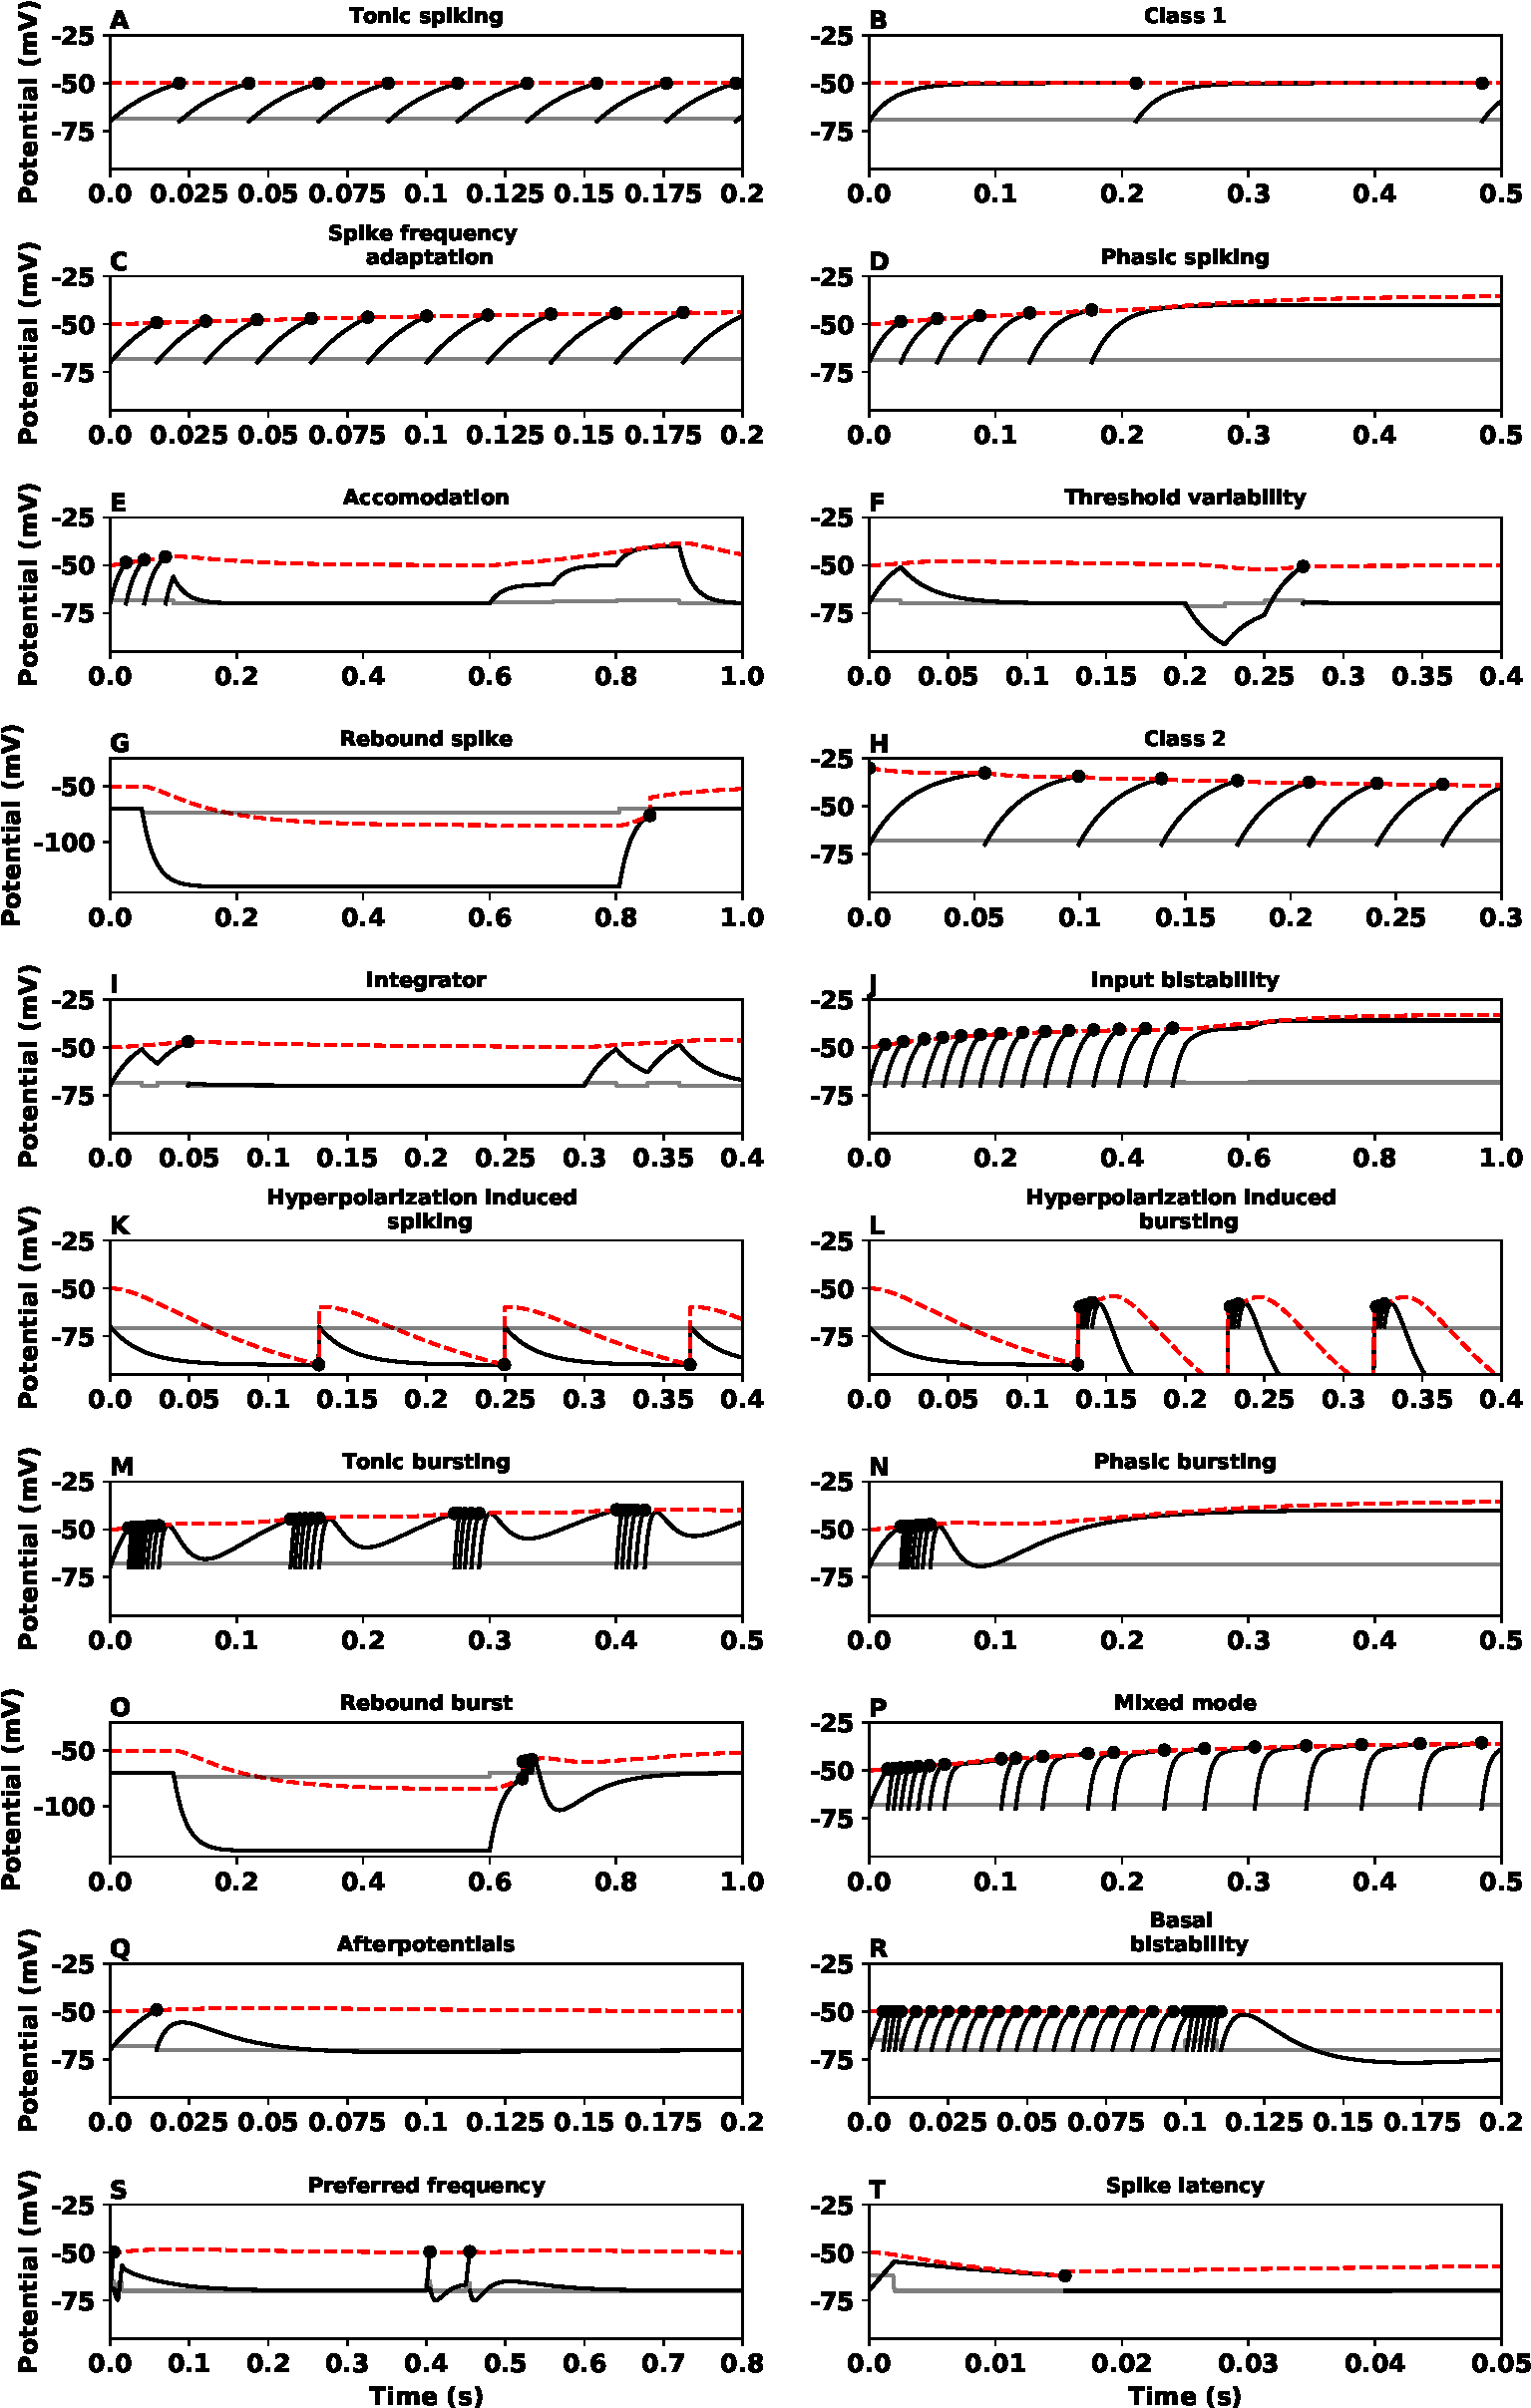
\includegraphics{figs/Figure01.pdf}
\caption{\textbf{Neural responses of MNN.} Black solid lines indicate
the membrane potential (\(V(t)\)), the red dashed lines show the
threshold potentials (\(\Theta(t)\)), and the gray lines the external
currents applied on each case. {\textbf{A}} tonic spiking, {\textbf{B}}
class \(1\), {\textbf{C}} spike frequency adaptation, {\textbf{D}}
phasic spiking, {\textbf{E}} accommodation, {\textbf{F}} threshold
variability, {\textbf{G}} rebound spike, {\textbf{H}} class \(2\),
{\textbf{I}} integrator, {\textbf{J}} input bistability, {\textbf{K}}
hyperpolarization induced spiking, {\textbf{L}} hyperpolarization
induced bursting, {\textbf{M}} tonic bursting, {\textbf{N}} phasic
bursting, {\textbf{O}} rebound burst, {\textbf{P}} mixed mode,
{\textbf{Q}} afterpotentials, {\textbf{R}} basal bistability,
{\textbf{S}} preferred frequency, {\textbf{T}} spike
latency.}\label{fig:1}
\end{figure}

\begin{figure}
\centering
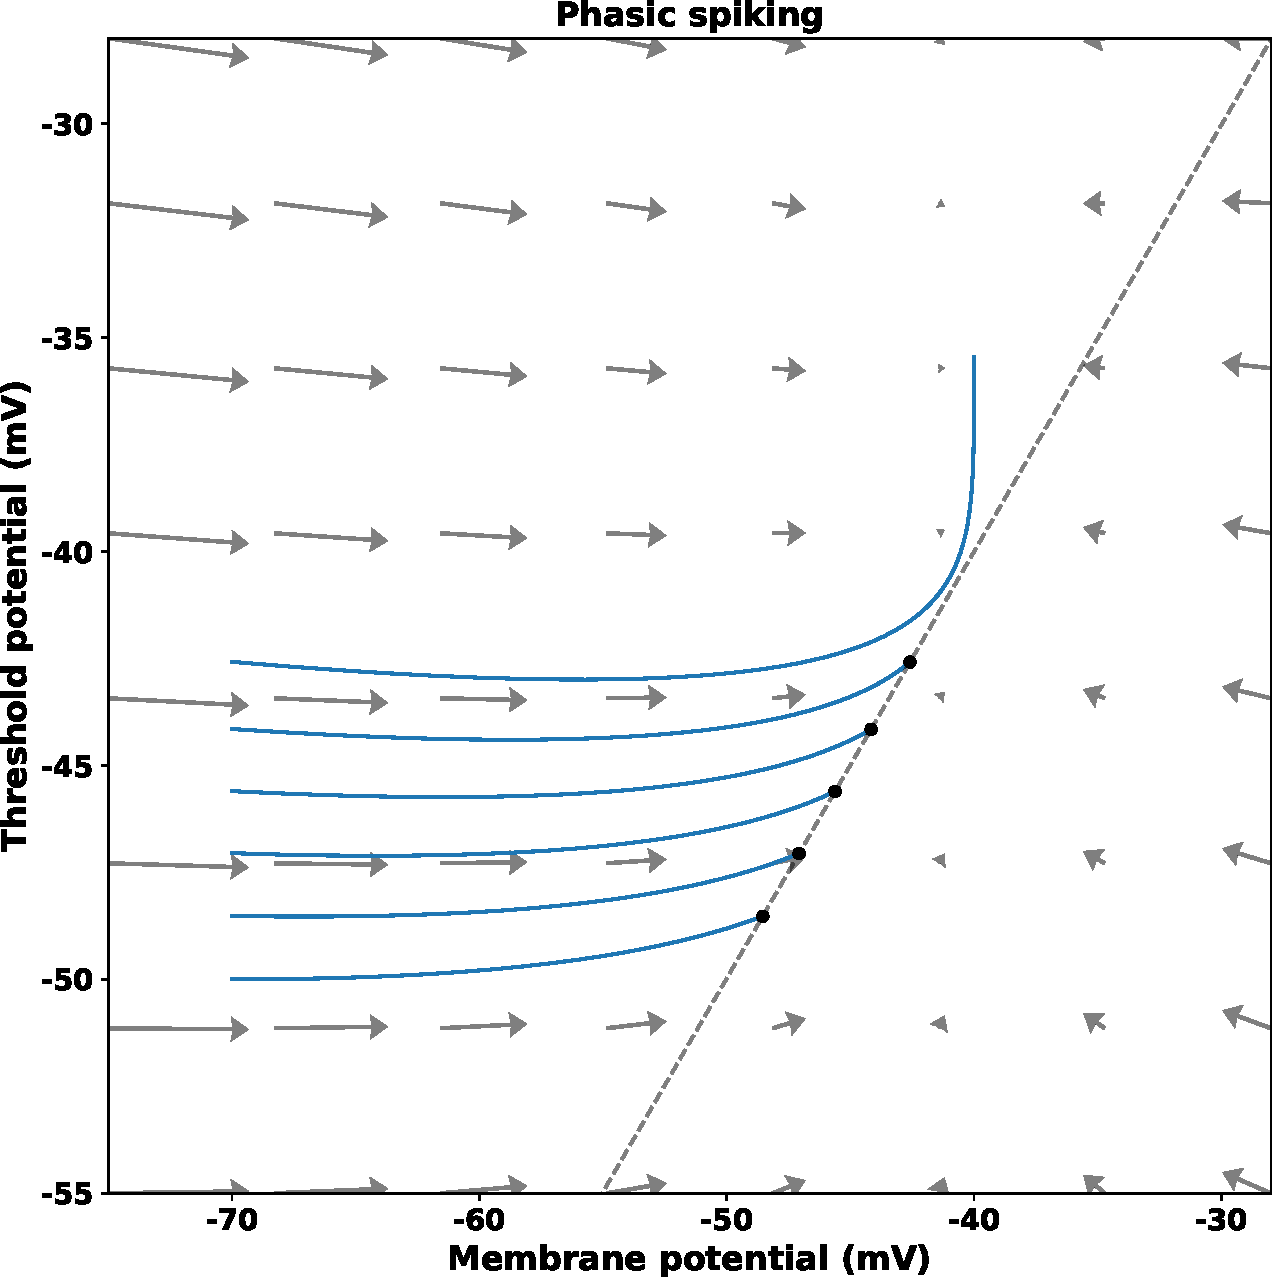
\includegraphics{figs/Figure02.pdf}
\caption{\textbf{Phase space of phasic spiking.} Blue solid lines
indicate the trajectories of the model in the phase spiking behavior
(Figure~~\ref{fig:1} D). The dashed line corresponds to
\(V(t) =  \Theta(t)\), and the black dots represent spike events. The
parameters for this simulation are the same as in Figure~~\ref{fig:1}
D.}\label{fig:2}
\end{figure}

\begin{figure}
\centering
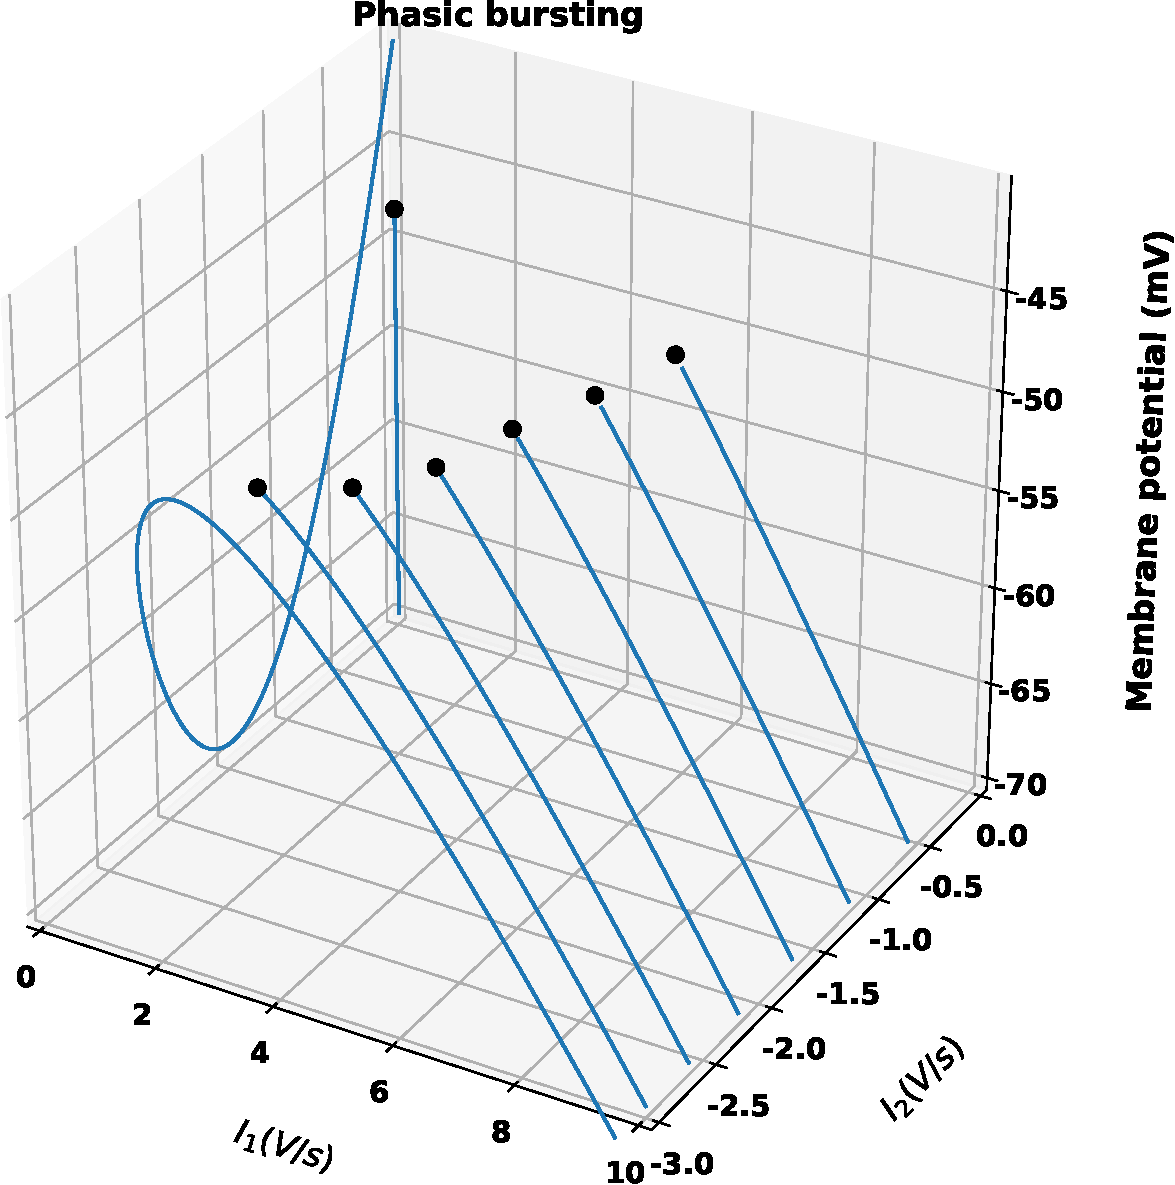
\includegraphics{figs/Figure03.pdf}
\caption{\textbf{Phase space of phasic bursting.} Blue solid lines
represent the trajectories of the system and the black dots indicate
spiking events. The parameters for this simulation are the same as in
Figure~~\ref{fig:1} N.}\label{fig:3}
\end{figure}

\section{Conclusion}\label{conclusion}

All figures in~\textcite{mihalas:2009} have been successfully replicated
with high fidelity. Overall, the whole reproducing process was smooth
and without obscure points since most of the parameters are provided in
the original article. Only the time intervals for which the external
current is applied to the model and the initial conditions are not
provided explicitly. Therefore, we had to extract that information from
figure \(1\) of the original article. To conclude, the
article~\autocite{mihalas:2009} has been successfully reproduced without
any discrepancy.

{\sffamily \small
  \printbibliography[title=References]
}
\end{document}
